\begin{figure}[tp]
\centering
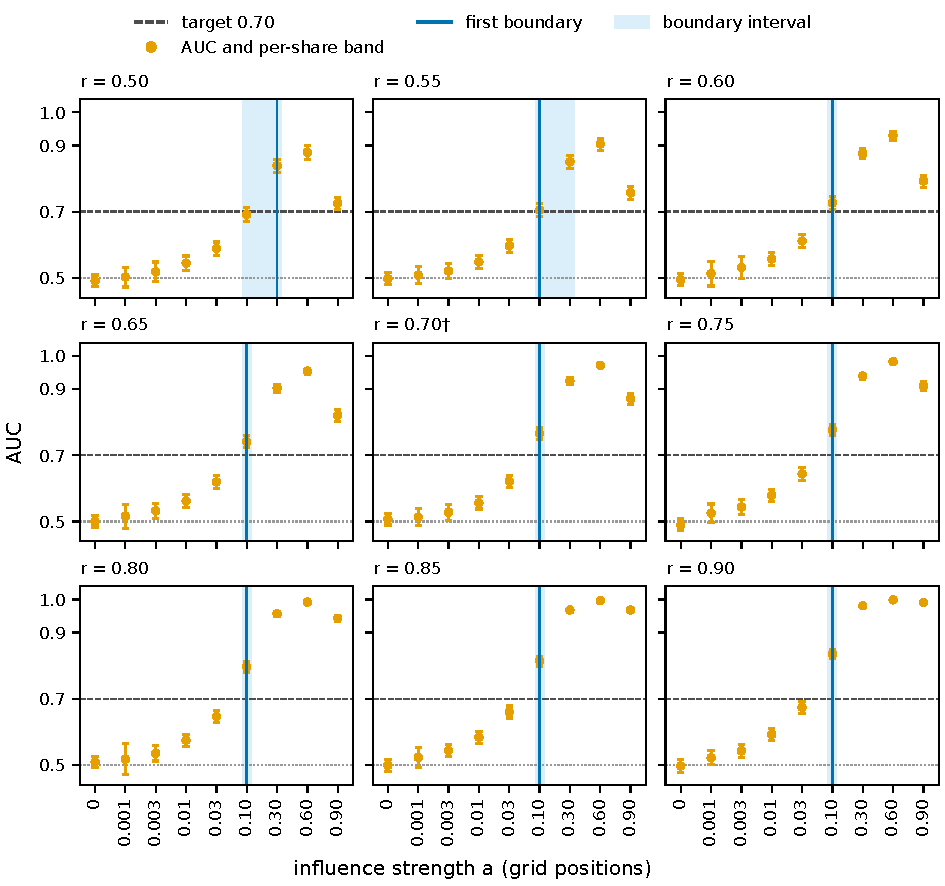
\includegraphics[width=\textwidth]{generated/J2_auc_profiles_A.pdf}
\caption{AUC profiles against autoregressive persistence (A). Vertical bars show per-share bands and crosses mark fit gaps. The target is \resultnum{j.target.r070}{0.70}. $\dag$ Examined during calibration.}\label{fig:auc-A}
\end{figure}
\begin{figure}[tp]
\centering
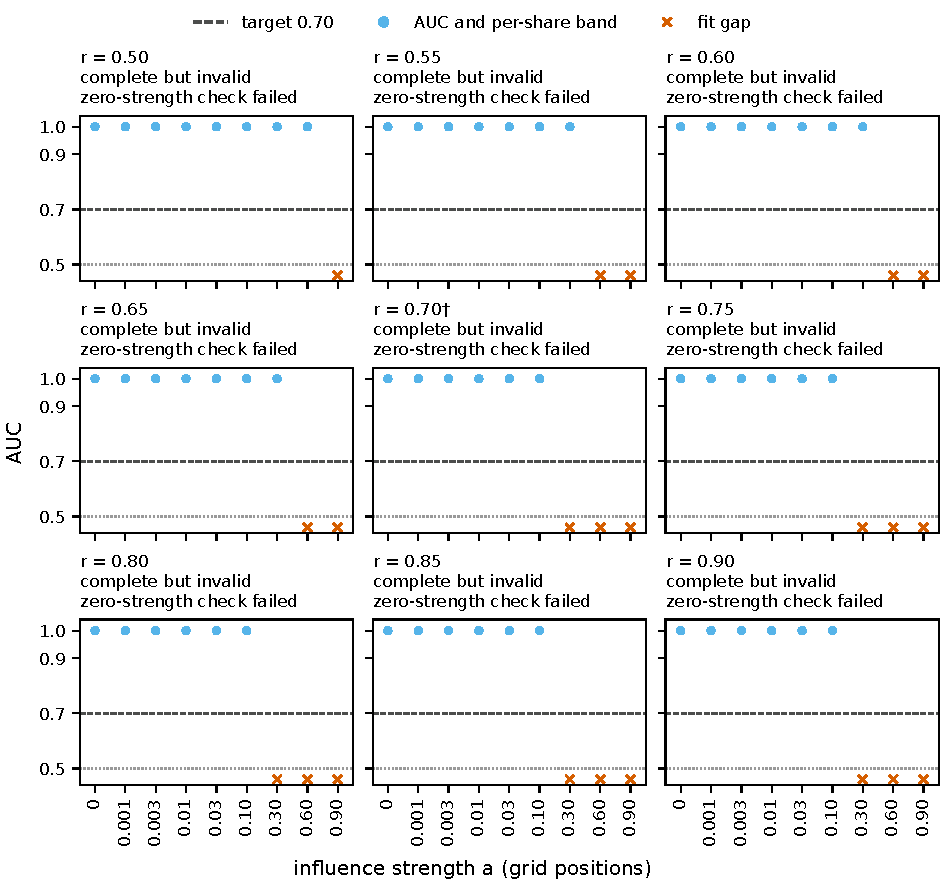
\includegraphics[width=\textwidth]{generated/J2_auc_profiles_C.pdf}
\caption{AUC profiles against autoregressive persistence with an altered response channel (C). Vertical bars show per-share bands and crosses mark fit gaps. The target is \resultnum{j.target.r070}{0.70}. $\dag$ Examined during calibration.}\label{fig:auc-C}
\end{figure}
\begin{figure}[tp]
\centering
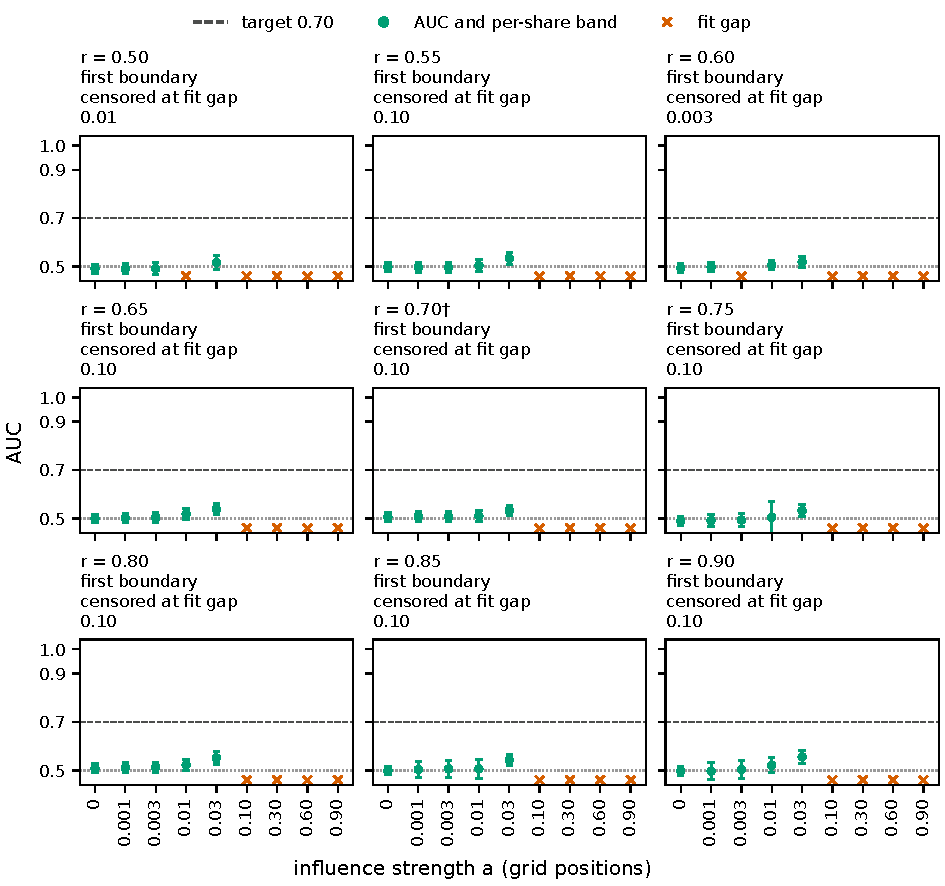
\includegraphics[width=\textwidth]{generated/J2_auc_profiles_D.pdf}
\caption{AUC profiles against state-dependent persistence (D). Vertical bars show per-share bands and crosses mark fit gaps. The target is \resultnum{j.target.r070}{0.70}. $\dag$ Examined during calibration.}\label{fig:auc-D}
\end{figure}
\begin{figure}[tp]
\centering
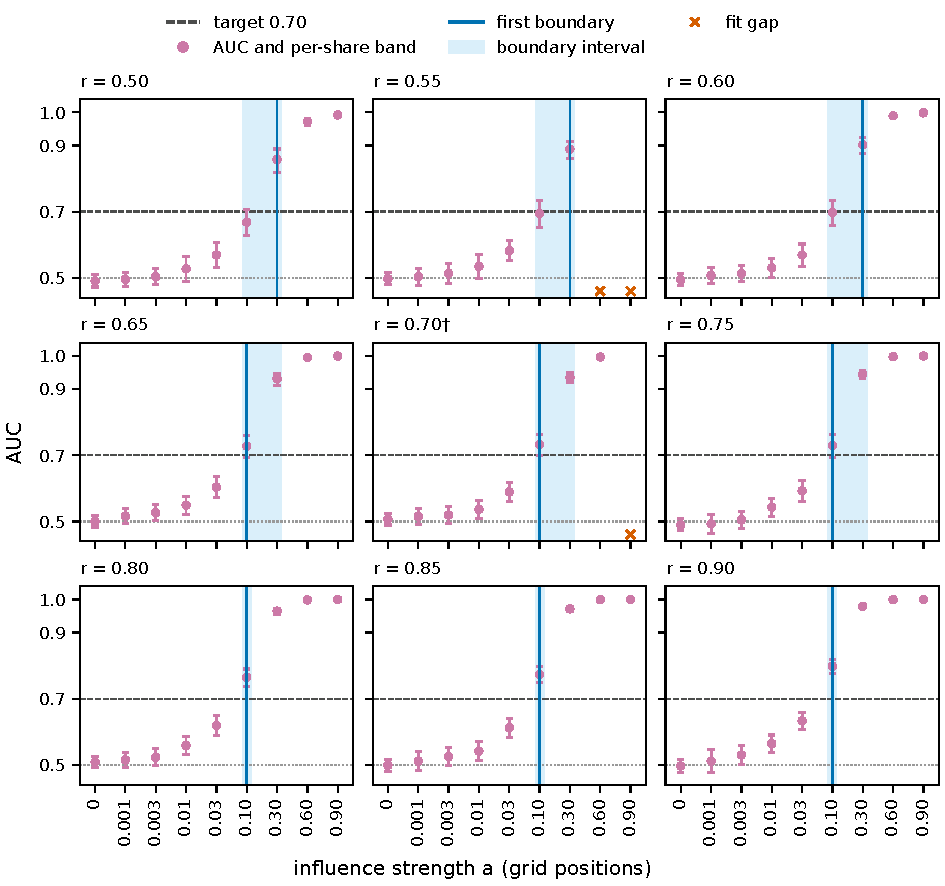
\includegraphics[width=\textwidth]{generated/J2_auc_profiles_E.pdf}
\caption{AUC profiles against mover--stayer persistence (E). Vertical bars show per-share bands and crosses mark fit gaps. The target is \resultnum{j.target.r070}{0.70}. $\dag$ Examined during calibration.}\label{fig:auc-E}
\end{figure}
